% FIG ch04-04b schematic labels (English)
\usetikzlibrary{positioning}
\begin{tikzpicture}
\node[anchor=south west,inner sep=0] (img) at (0,0) {%
  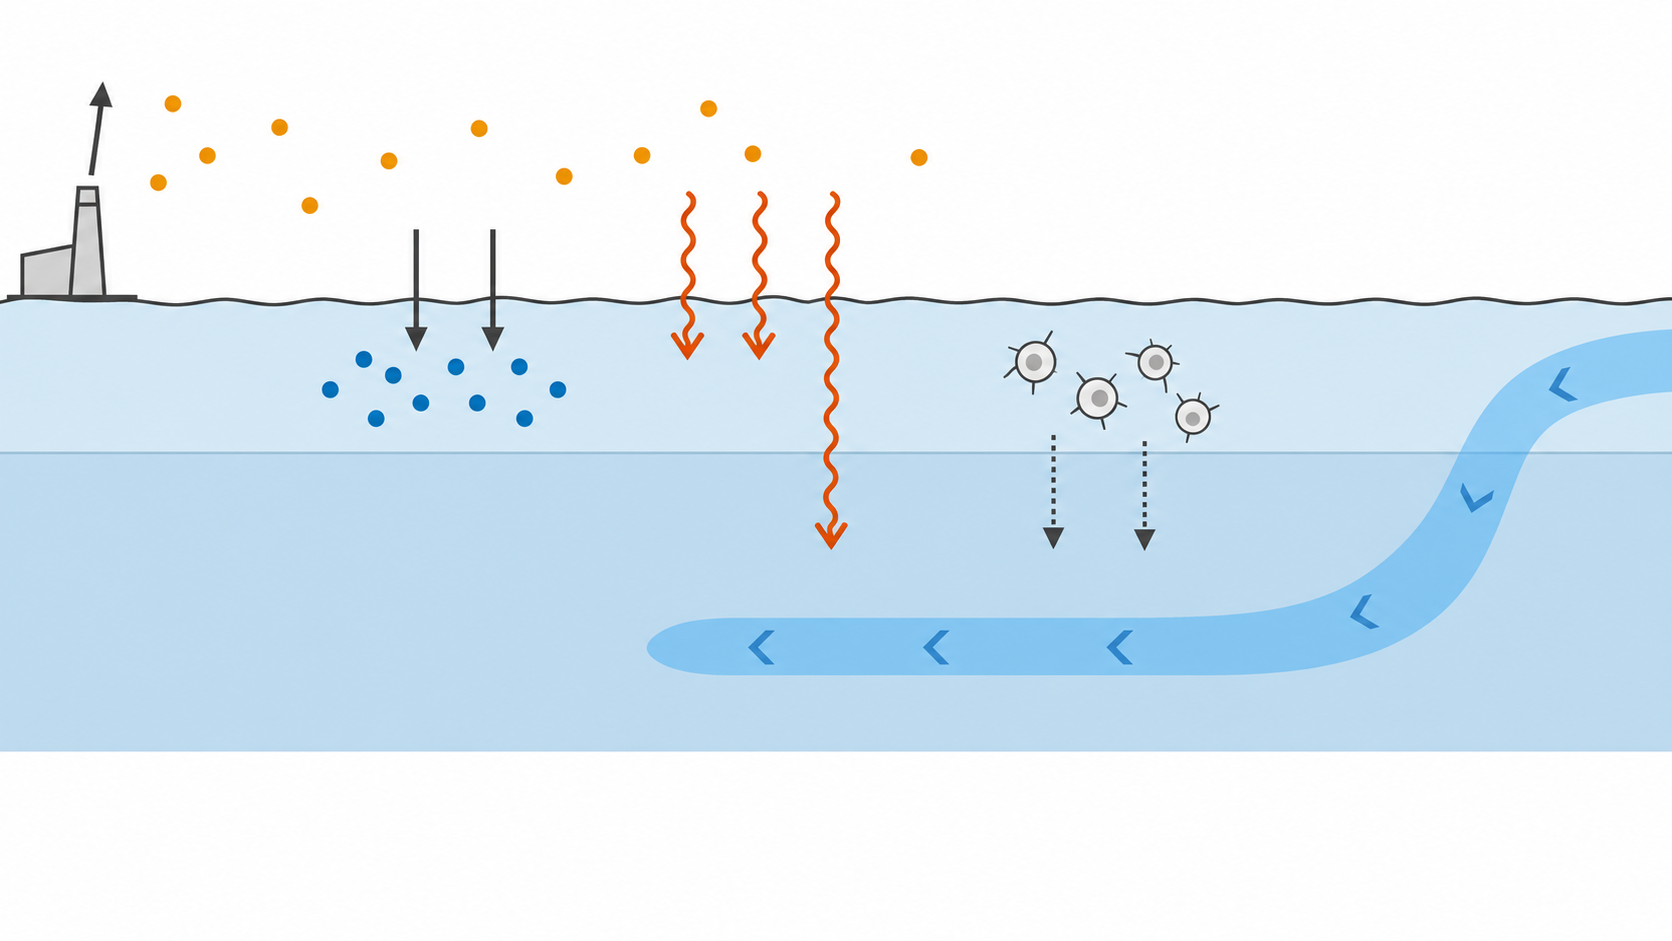
\includegraphics[width=\linewidth]{figures/ch04/ch04-04b-schematic-base.png}};
\begin{scope}[x={(img.south east)},y={(img.north west)},font=\sffamily\small]
  \node at (0.92,0.90) {Atmosphere};
  \node at (0.92,0.66) {Mixed layer};
  \node at (0.92,0.35) {Ocean interior};
  \node[align=left] at (0.06,0.93) {Anthropogenic emissions};
  \node at (0.30,0.88) {CO\textsubscript{2}};
  \node at (0.33,0.70) {Air--sea gas exchange};
  \node at (0.30,0.60) {Dissolved inorganic carbon};
  \node at (0.55,0.70) {Heat uptake};
  \node[align=center] at (0.80,0.45) {Sinking and transport\\of water};
  \node at (0.48,0.62) {Phytoplankton};
  \node[align=center] at (0.48,0.42) {Sinking particles\\(biological pump)};
  \node[align=center,font=\scriptsize] at (0.50,0.04) {%
    Legend: carbon flux / heat flux / water transport / sinking particles};
\end{scope}
\end{tikzpicture}
